\documentclass[11pt]{beamer}

%%% \mode must be on a line by its own, without comment or whitespace!
%%% \mode sets the mode to presentation. So if the mode is presentation the slides after are shown
%%% if the mode is not presentation (but article or handout) they are not shown
\mode<presentation>

\usetheme{Warsaw}
\usepackage[utf8]{inputenc}
\usepackage[english]{babel}
\usepackage{amsmath}
\usepackage{amsfonts}
\usepackage{amssymb}
\usepackage{graphicx}
\usepackage{xspace}

\author{Guus Bonnema}
\title{Architecture}
%\setbeamercovered{transparent} 
%\setbeamertemplate{navigation symbols}{} 
%\logo{} 
\institute{Open University\\team033\\Guus Bonnema, Stefan Versluys, Jeroen Kleijn} 
\date{December 06, 2014} 
\subject{main views} 

\begin{document}

\newcommand{\Noc}{\textsc{NoC}\xspace}

\begin{frame}
\titlepage
\end{frame}

\begin{frame}
	\begin{itemize}
		\item<1-> Basic design principles \uncover<2->{\color{red} Do you agree?}
		\item<1-> System partitioning \uncover<3->{\color{red} Some queries}
		\item<1-> System dynamics \uncover<4->{\color{red} What we envision}
	\end{itemize}
\end{frame}

\begin{frame}{Design guidelines}

	\uncover<6>{\center{\color{blue} This will drive our decisions:}{\color{red} Do you agree?}}
	
	\vspace{2em}
	
	\uncover<1-> {\color{black} We need some design guidelines to decide on stuff}

	\begin{description}
	\item<2,6>[\bf Portability] {\color{blue} \it 1st main goal:} Portability is a leading requirement.
	
	\item<3,6>[\bf Ease of use / install] {\color{blue} \it 2nd main goal:} Assist in the design of \Noc + Promote tools to outsiders
	
	\item<4,6>[\bf Maintainability] {\color{blue} \it 3rd main goal:} A primary requirement 
	
	\item<5,6>[\bf Performance] {\color{blue} \it Follows} For all acceptable performance (subjective) 
	
	\end{description}
	
\end{frame}

\begin{frame}{Partitioning the system}
	\uncover<1>{\huge Design Tool Scope}
	\uncover<2>{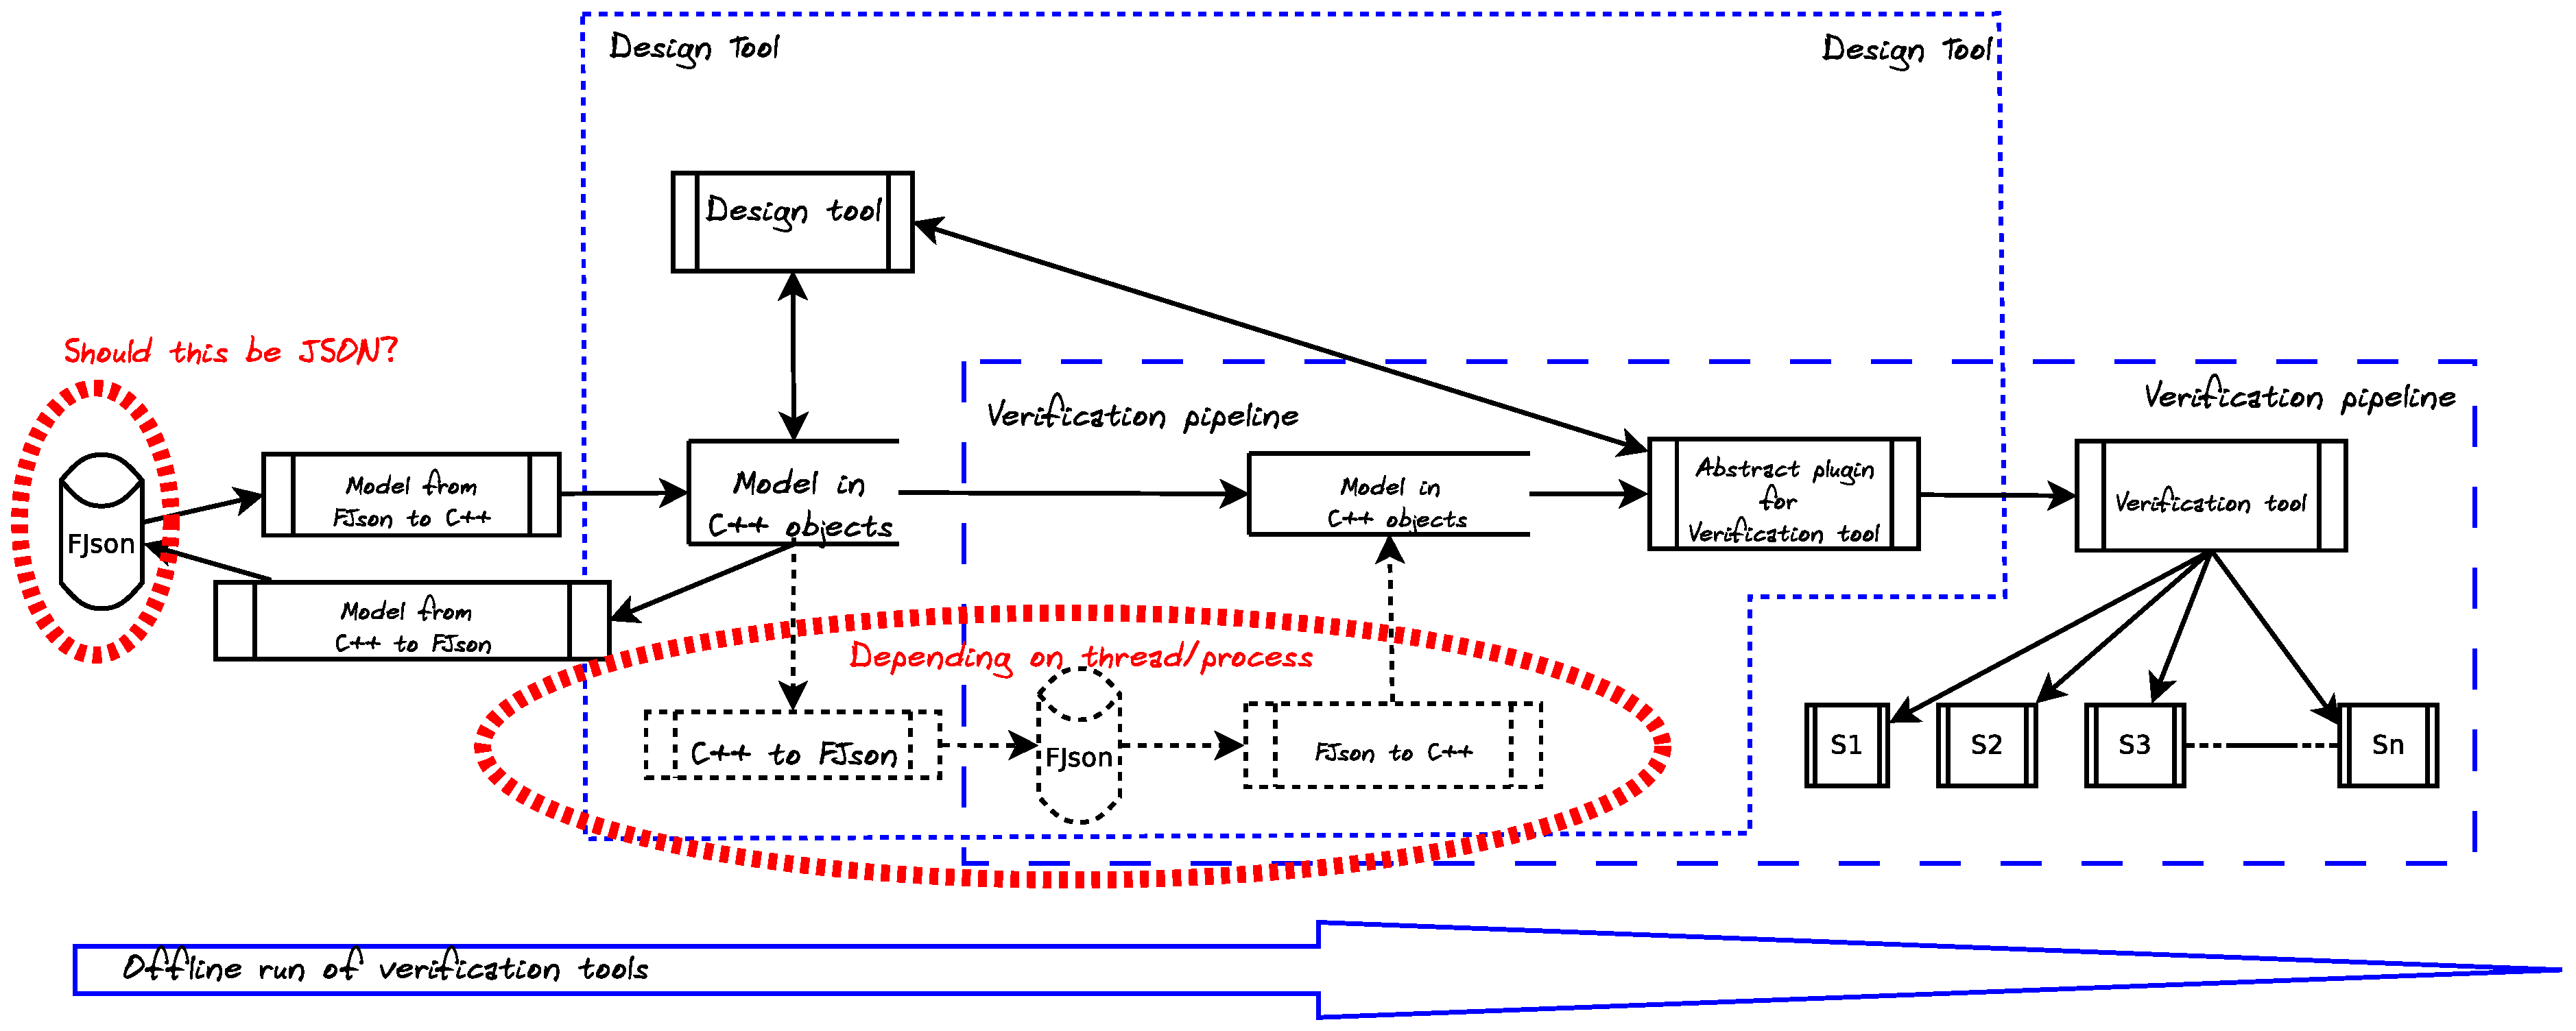
\includegraphics[width=.95\linewidth]{architecture-tool-scope}}
\end{frame}

\begin{frame}{System dynamics}
	\uncover<1>{\huge Design Tool dynamics}
	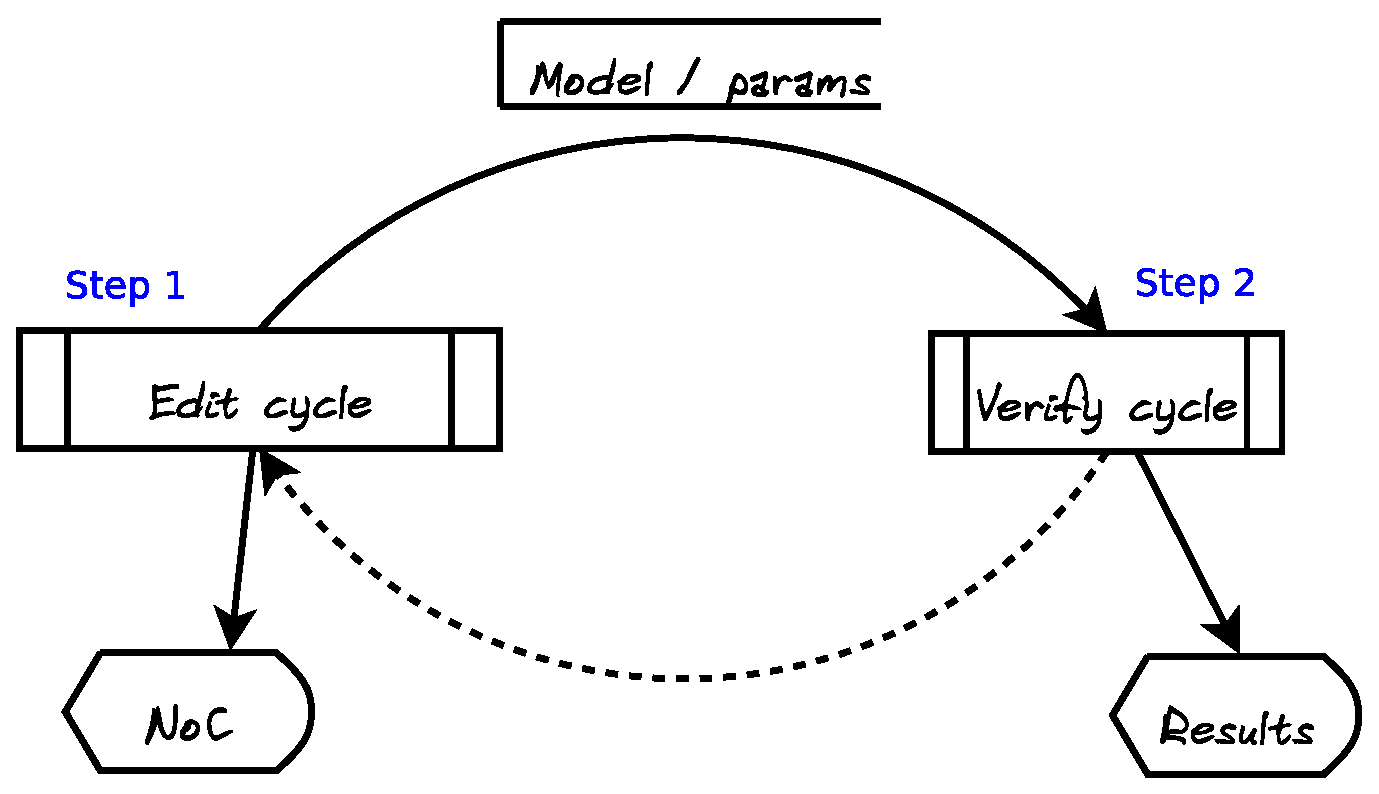
\includegraphics[width=.95\linewidth]{architecture-dynamic-overview}<2>
	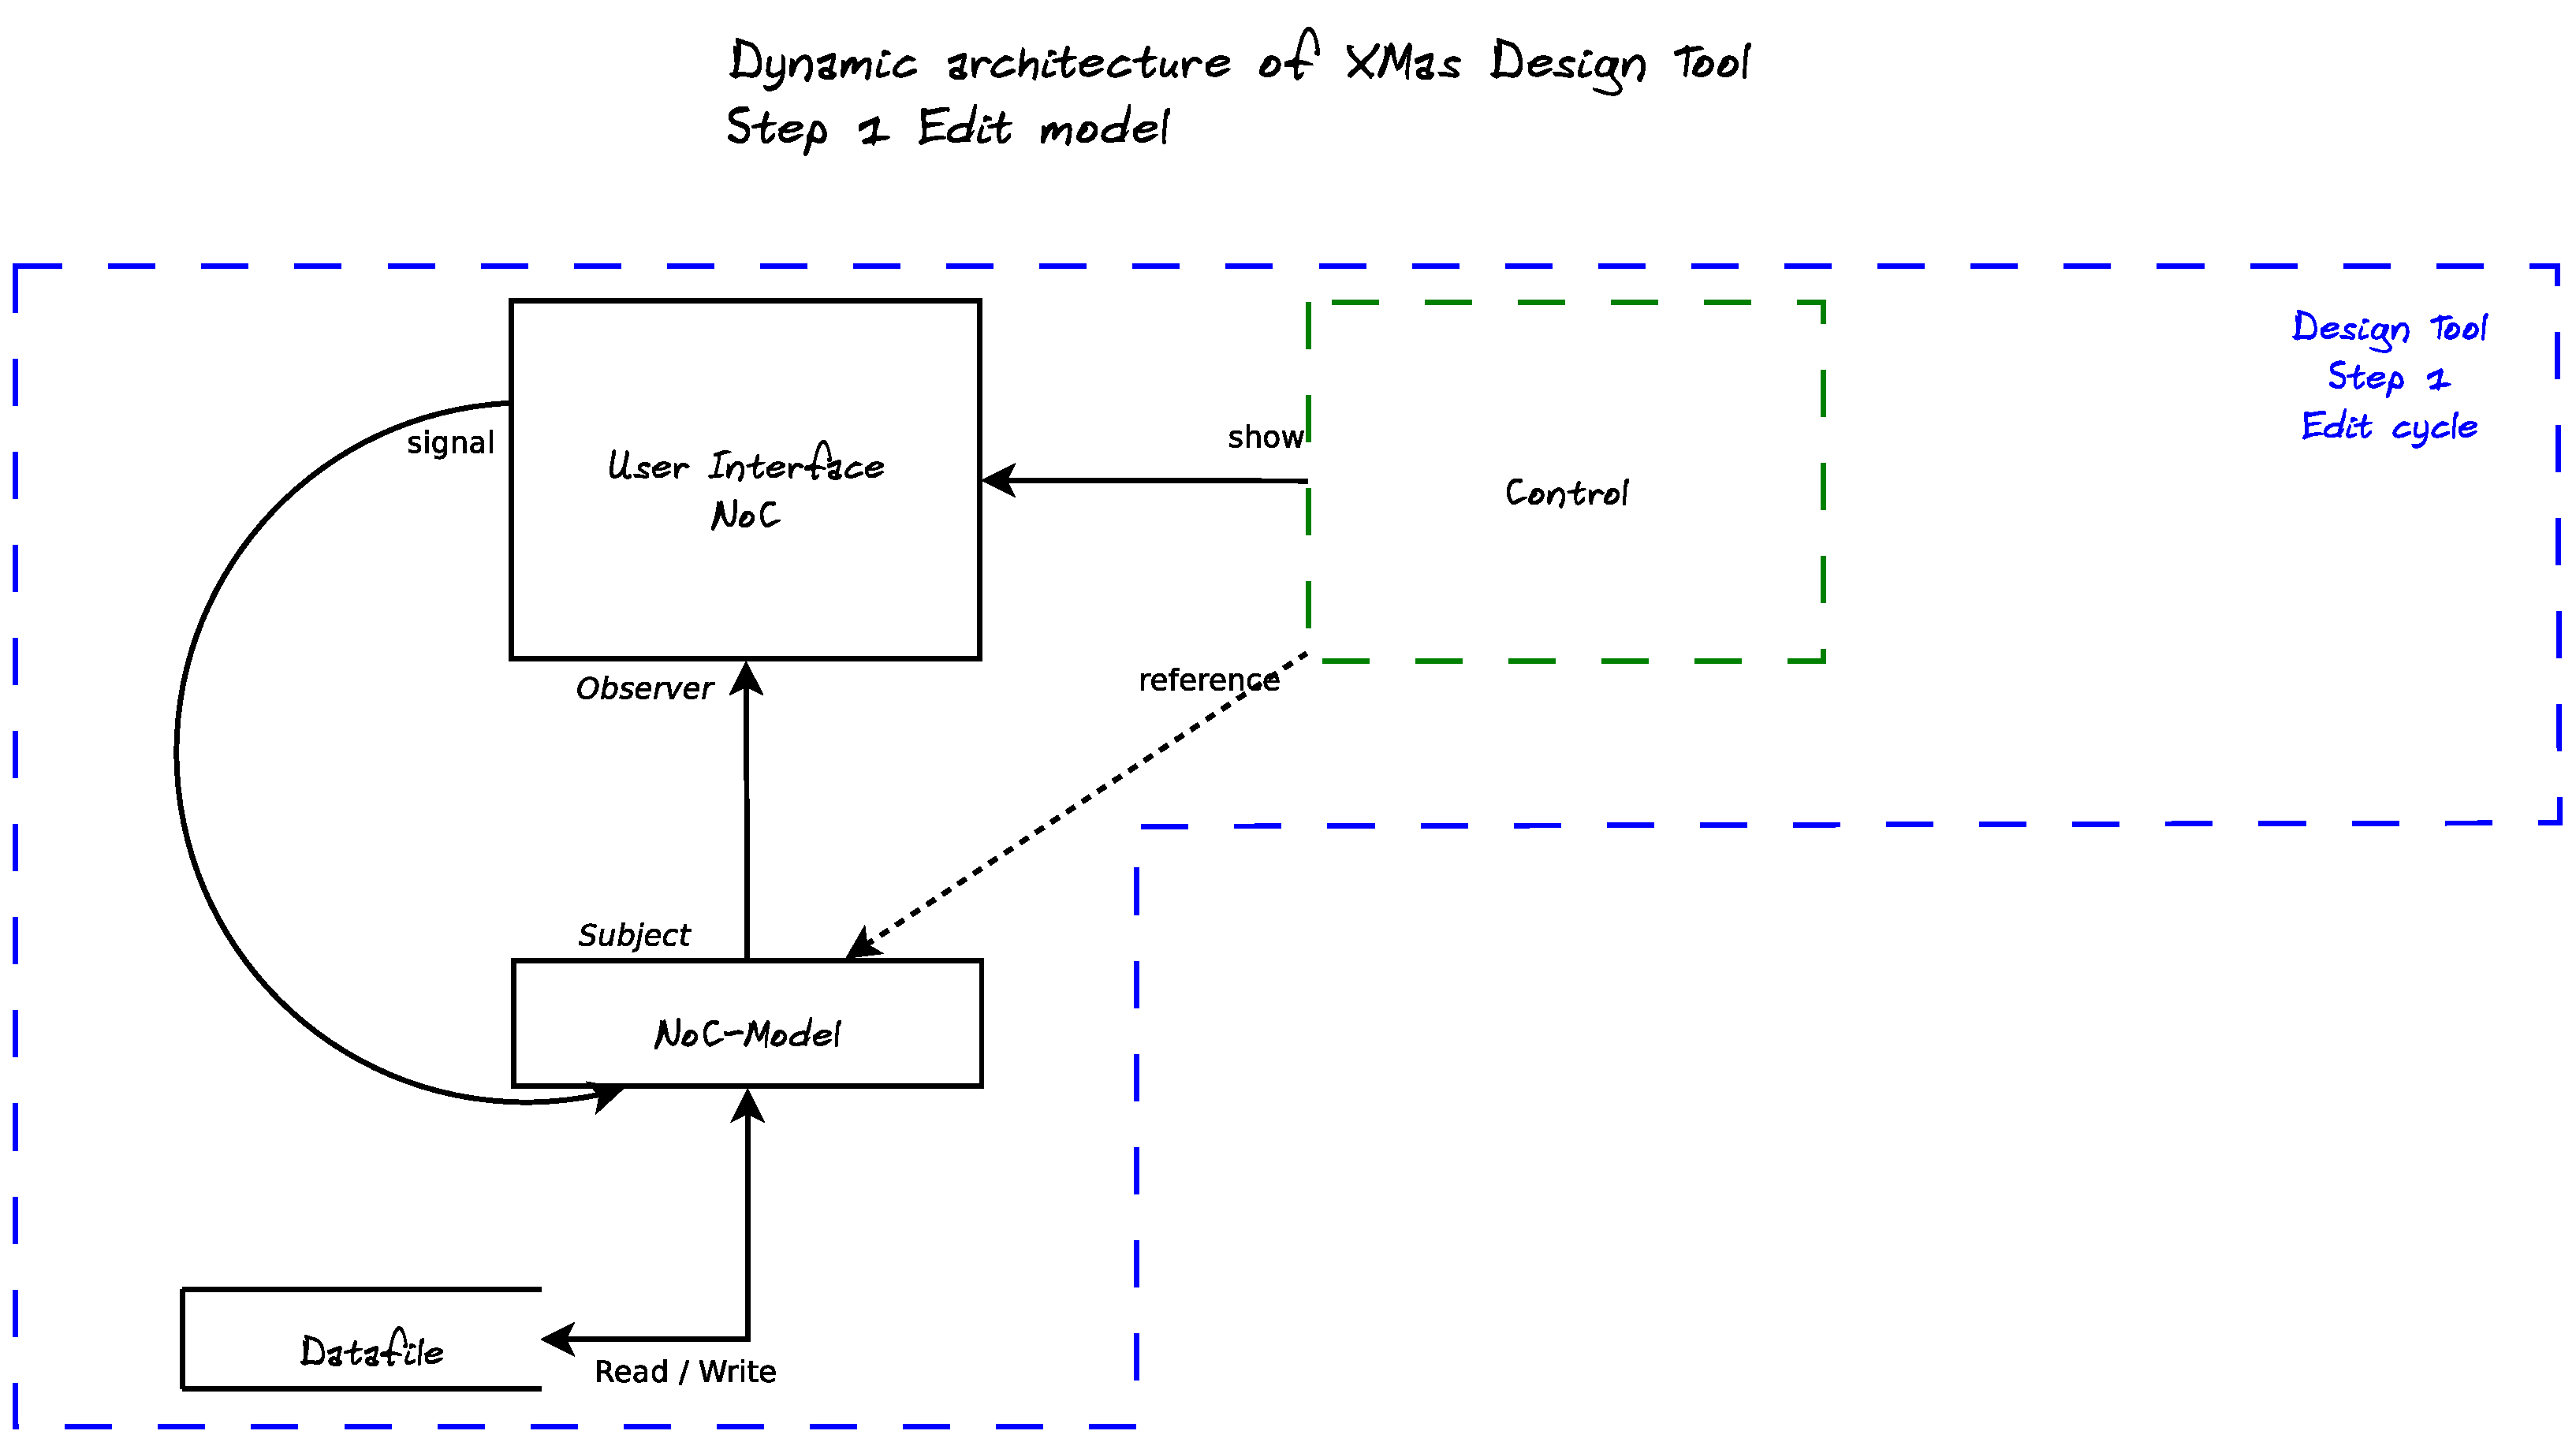
\includegraphics[width=.95\linewidth]{1-architecture-dynamic}<3> 
	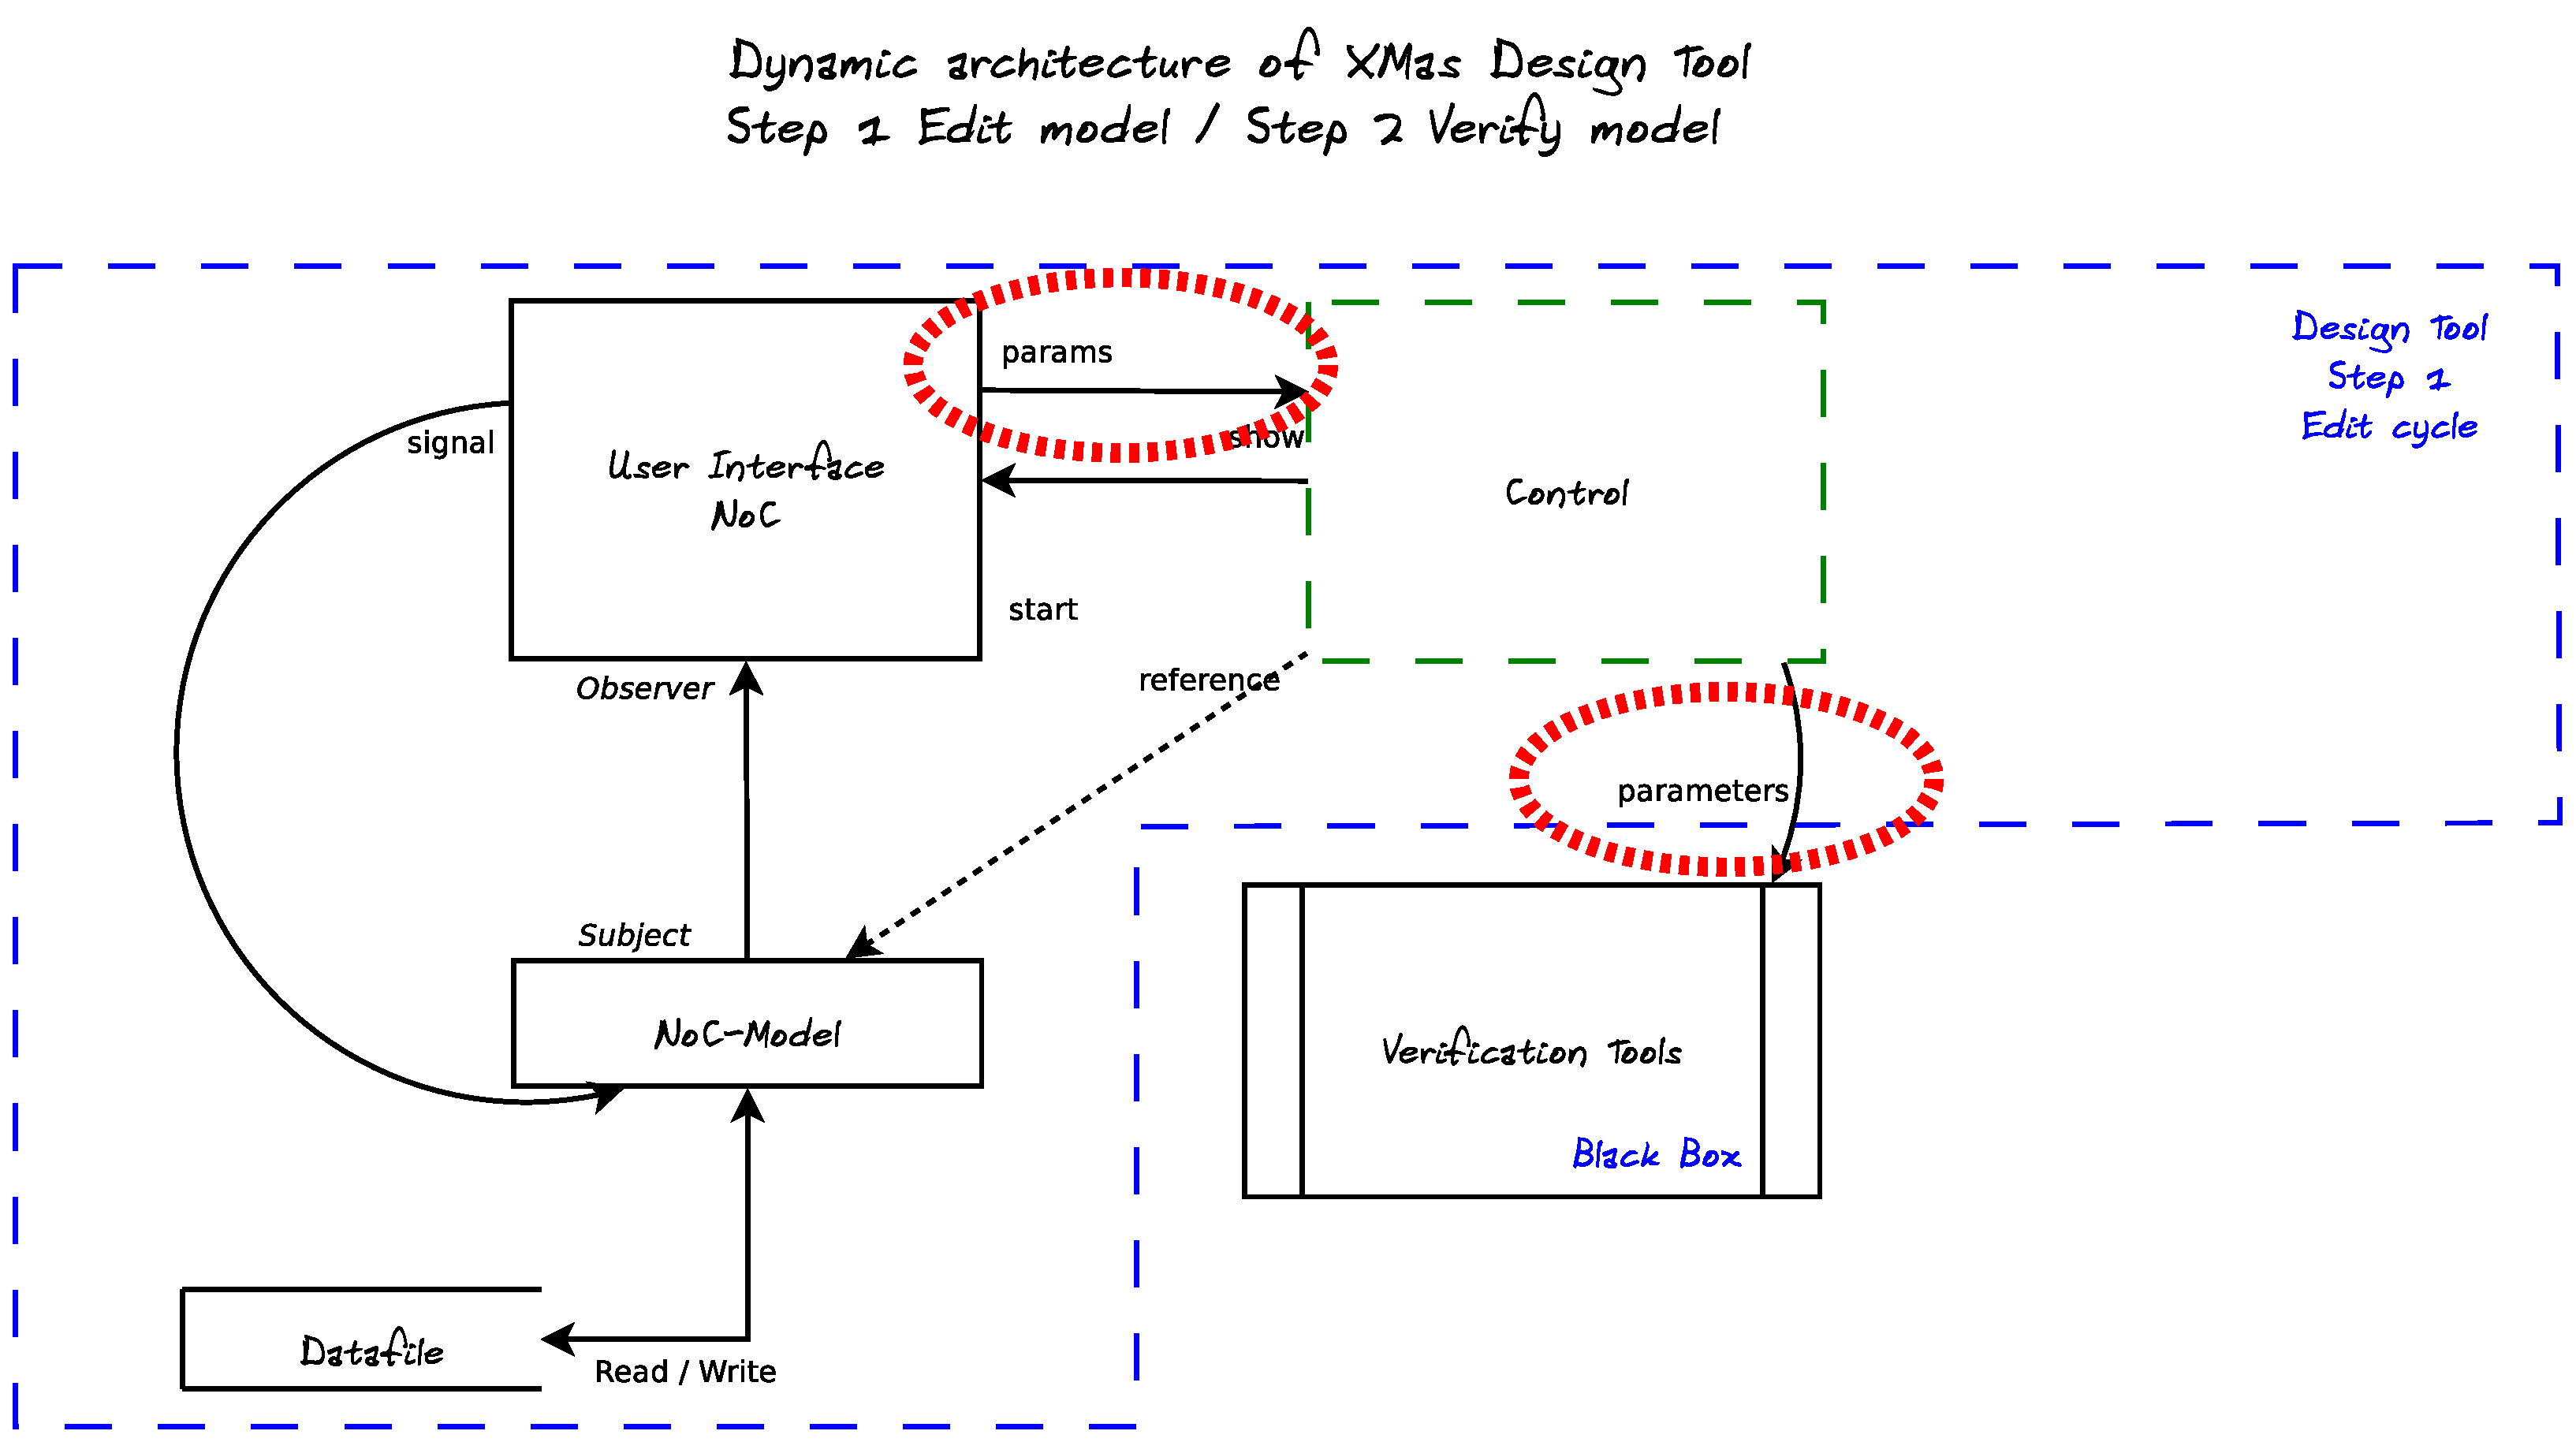
\includegraphics[width=.95\linewidth]{1a-architecture-dynamic}<4>
	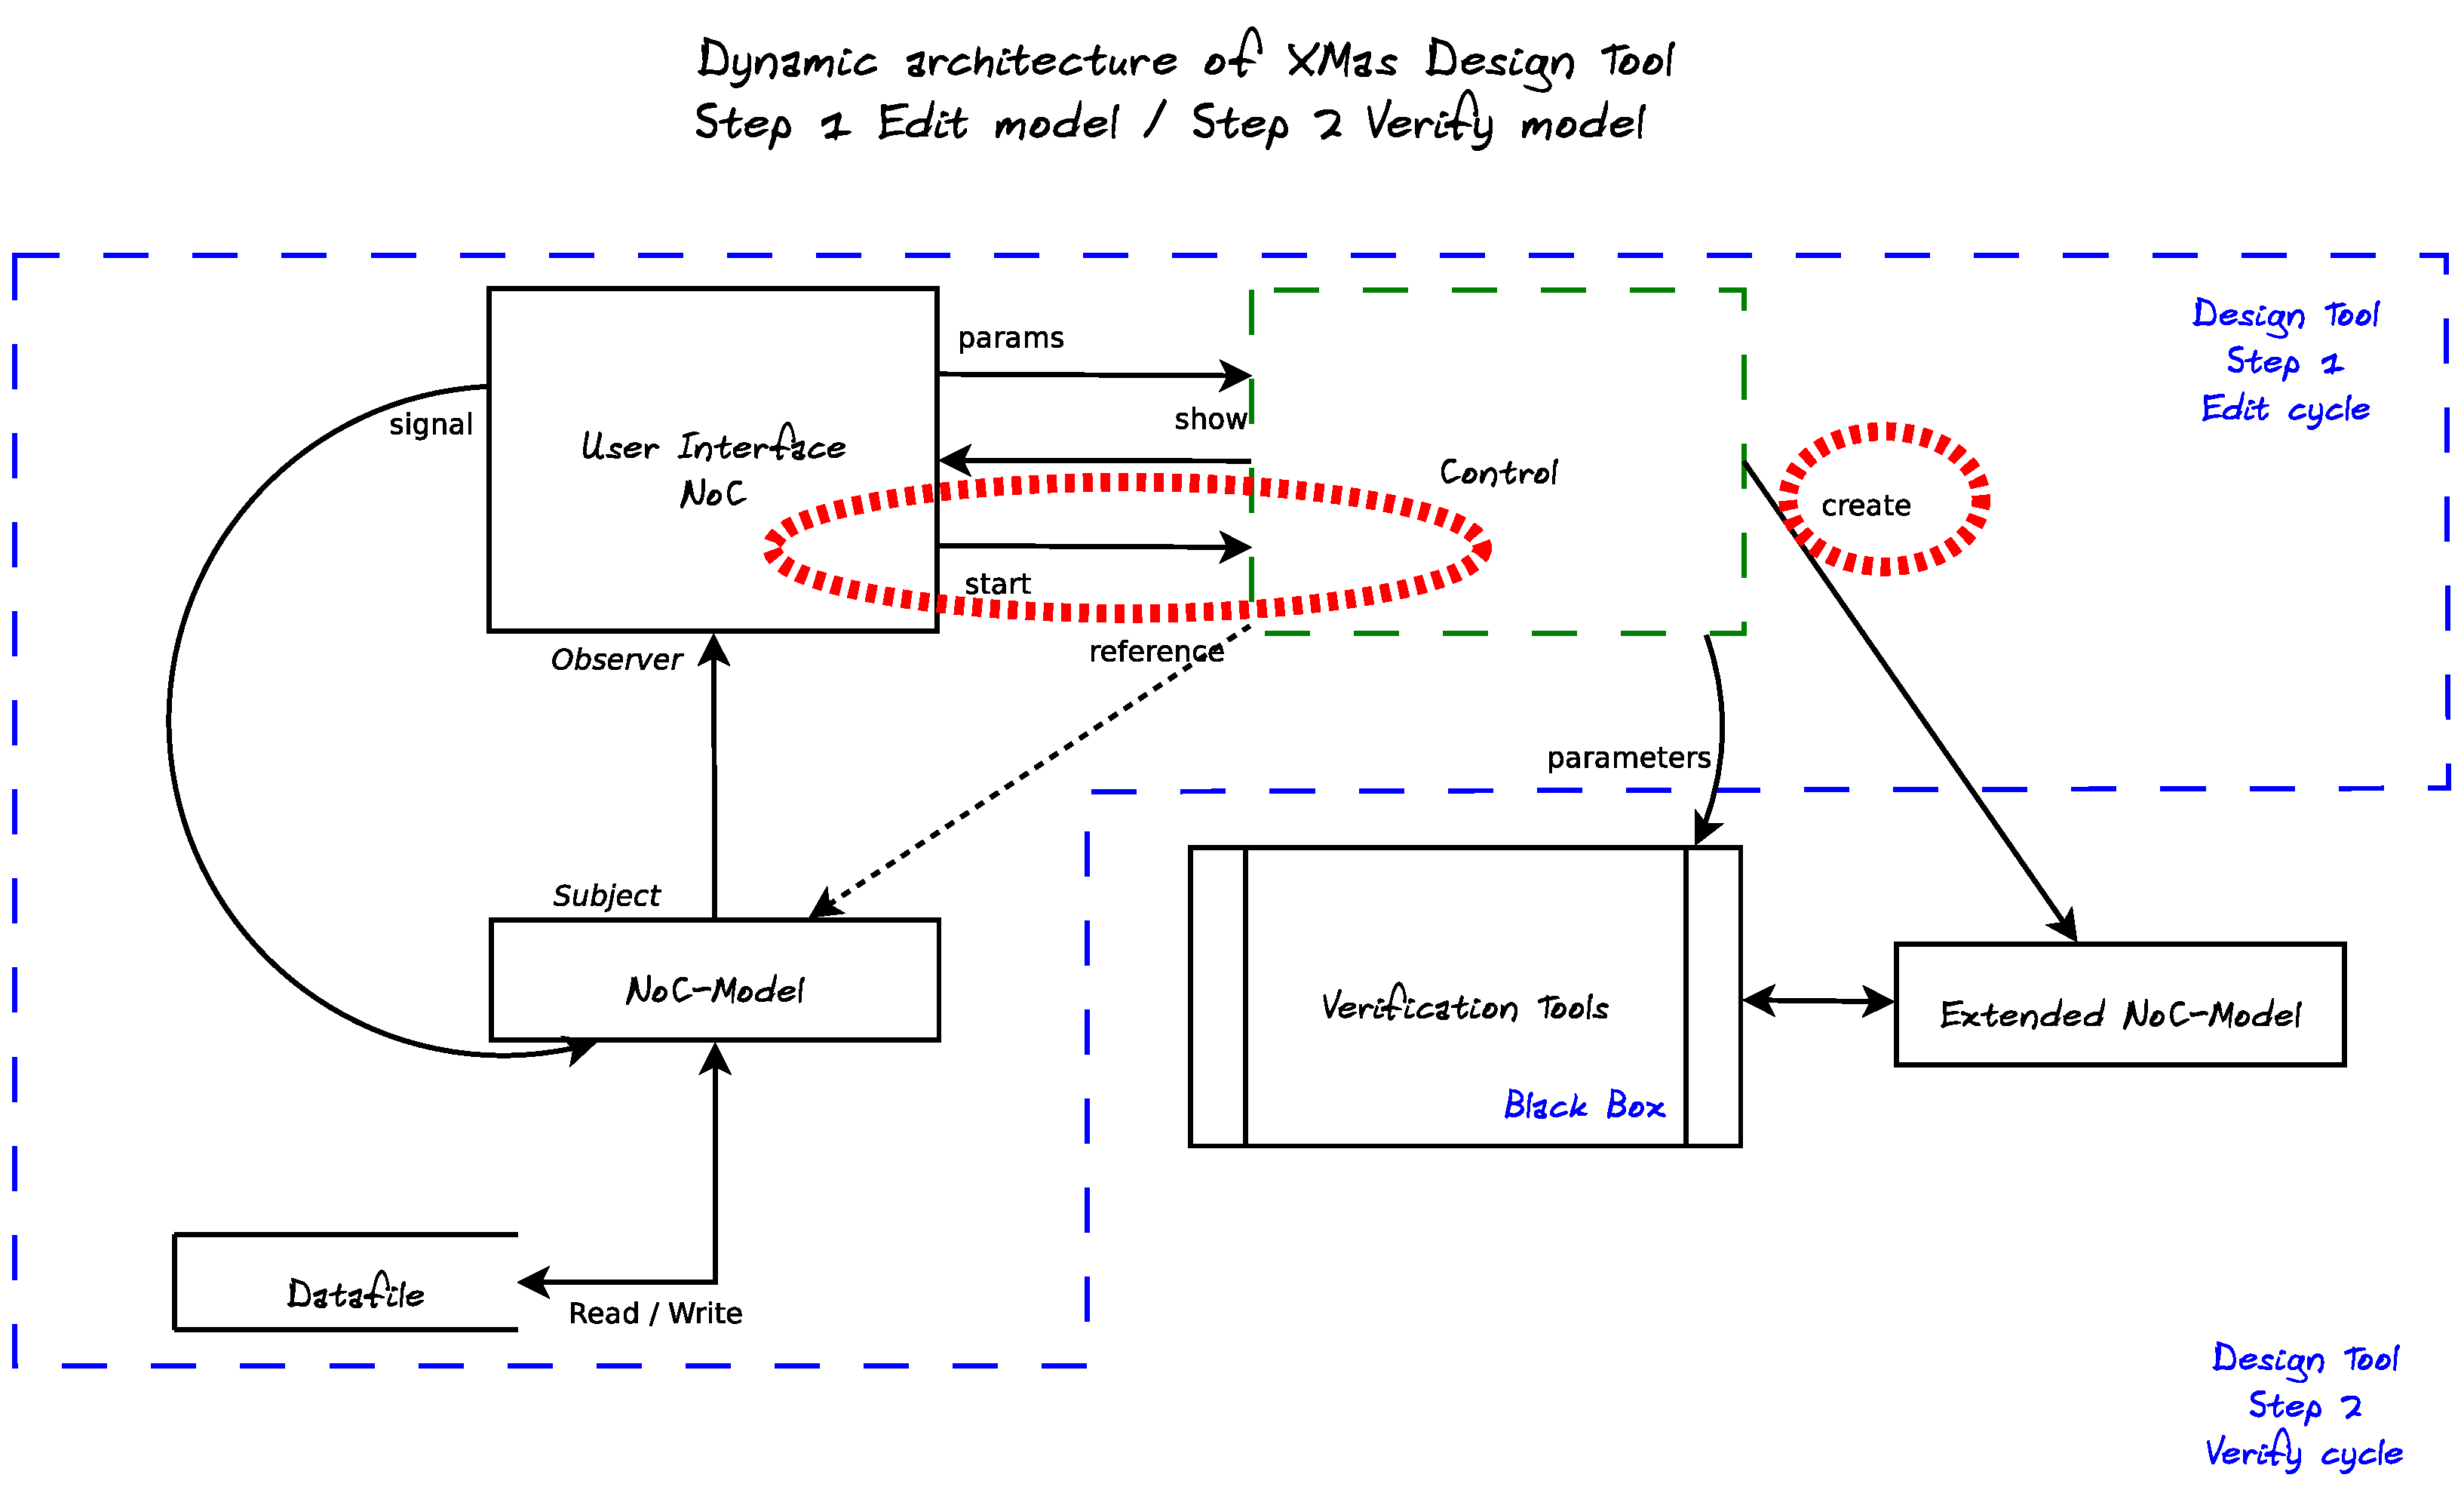
\includegraphics[width=.95\linewidth]{1b1-architecture-dynamic}<5>
	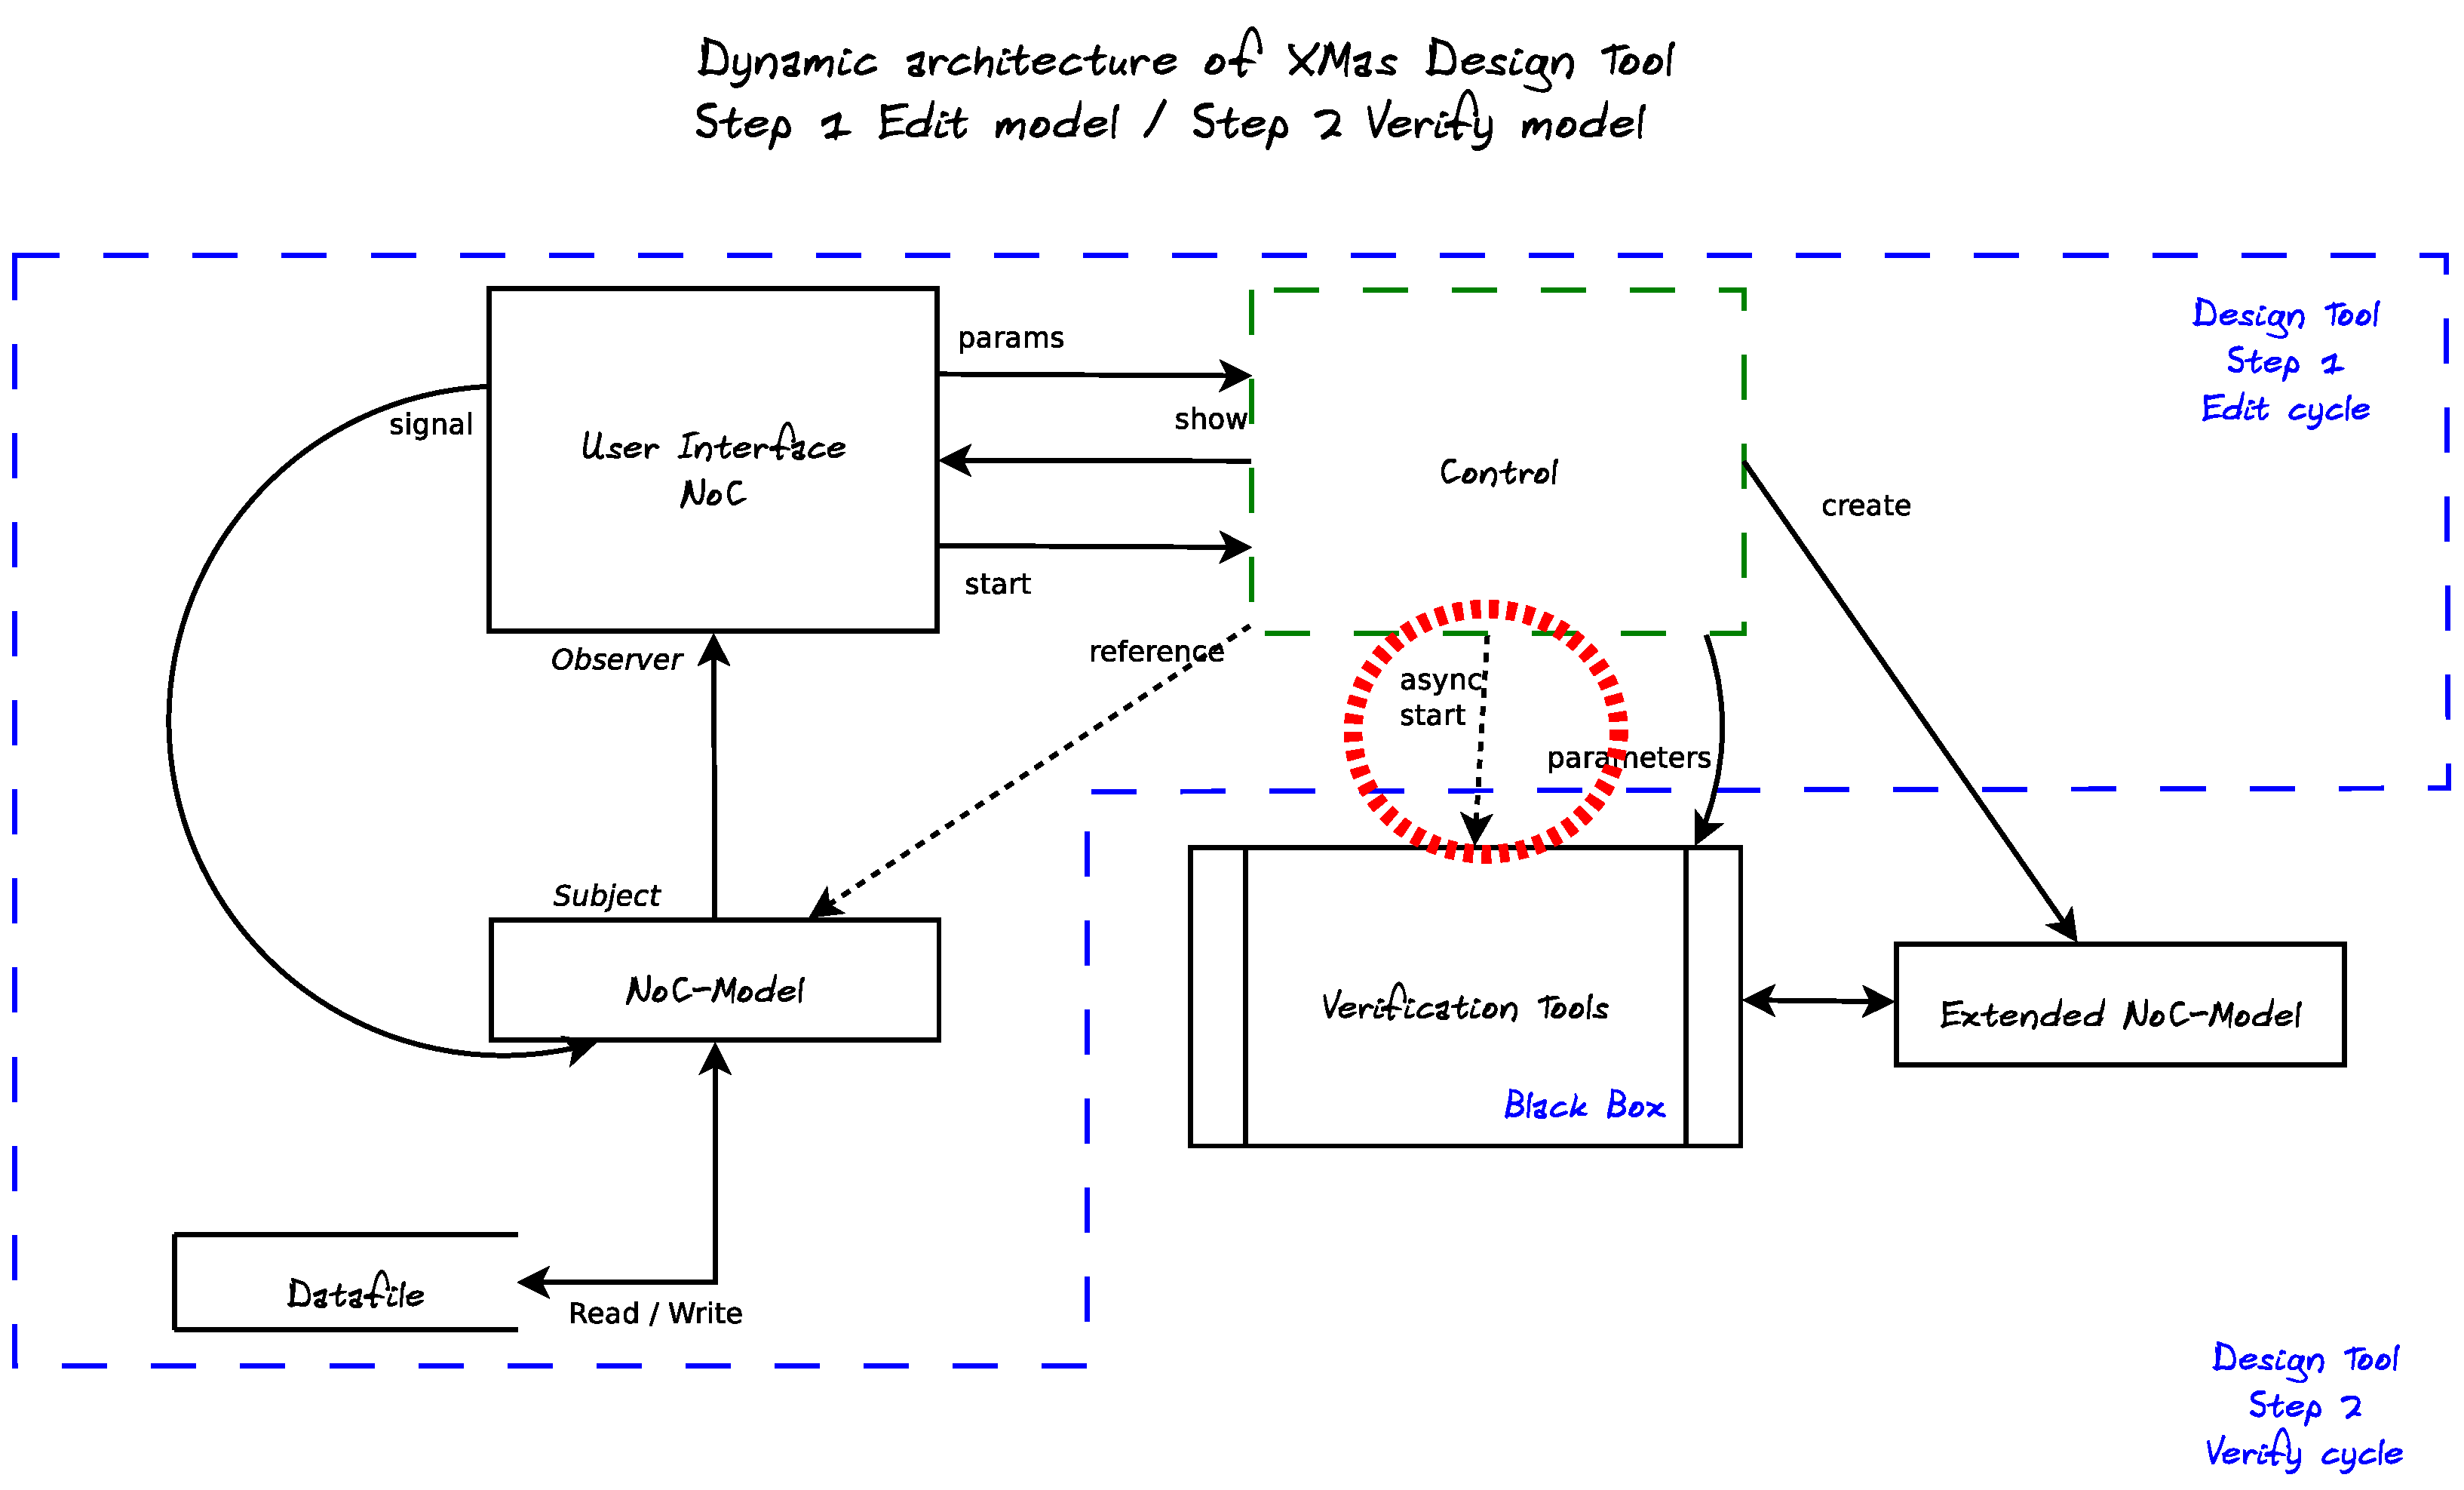
\includegraphics[width=.95\linewidth]{1b2-architecture-dynamic}<6>
	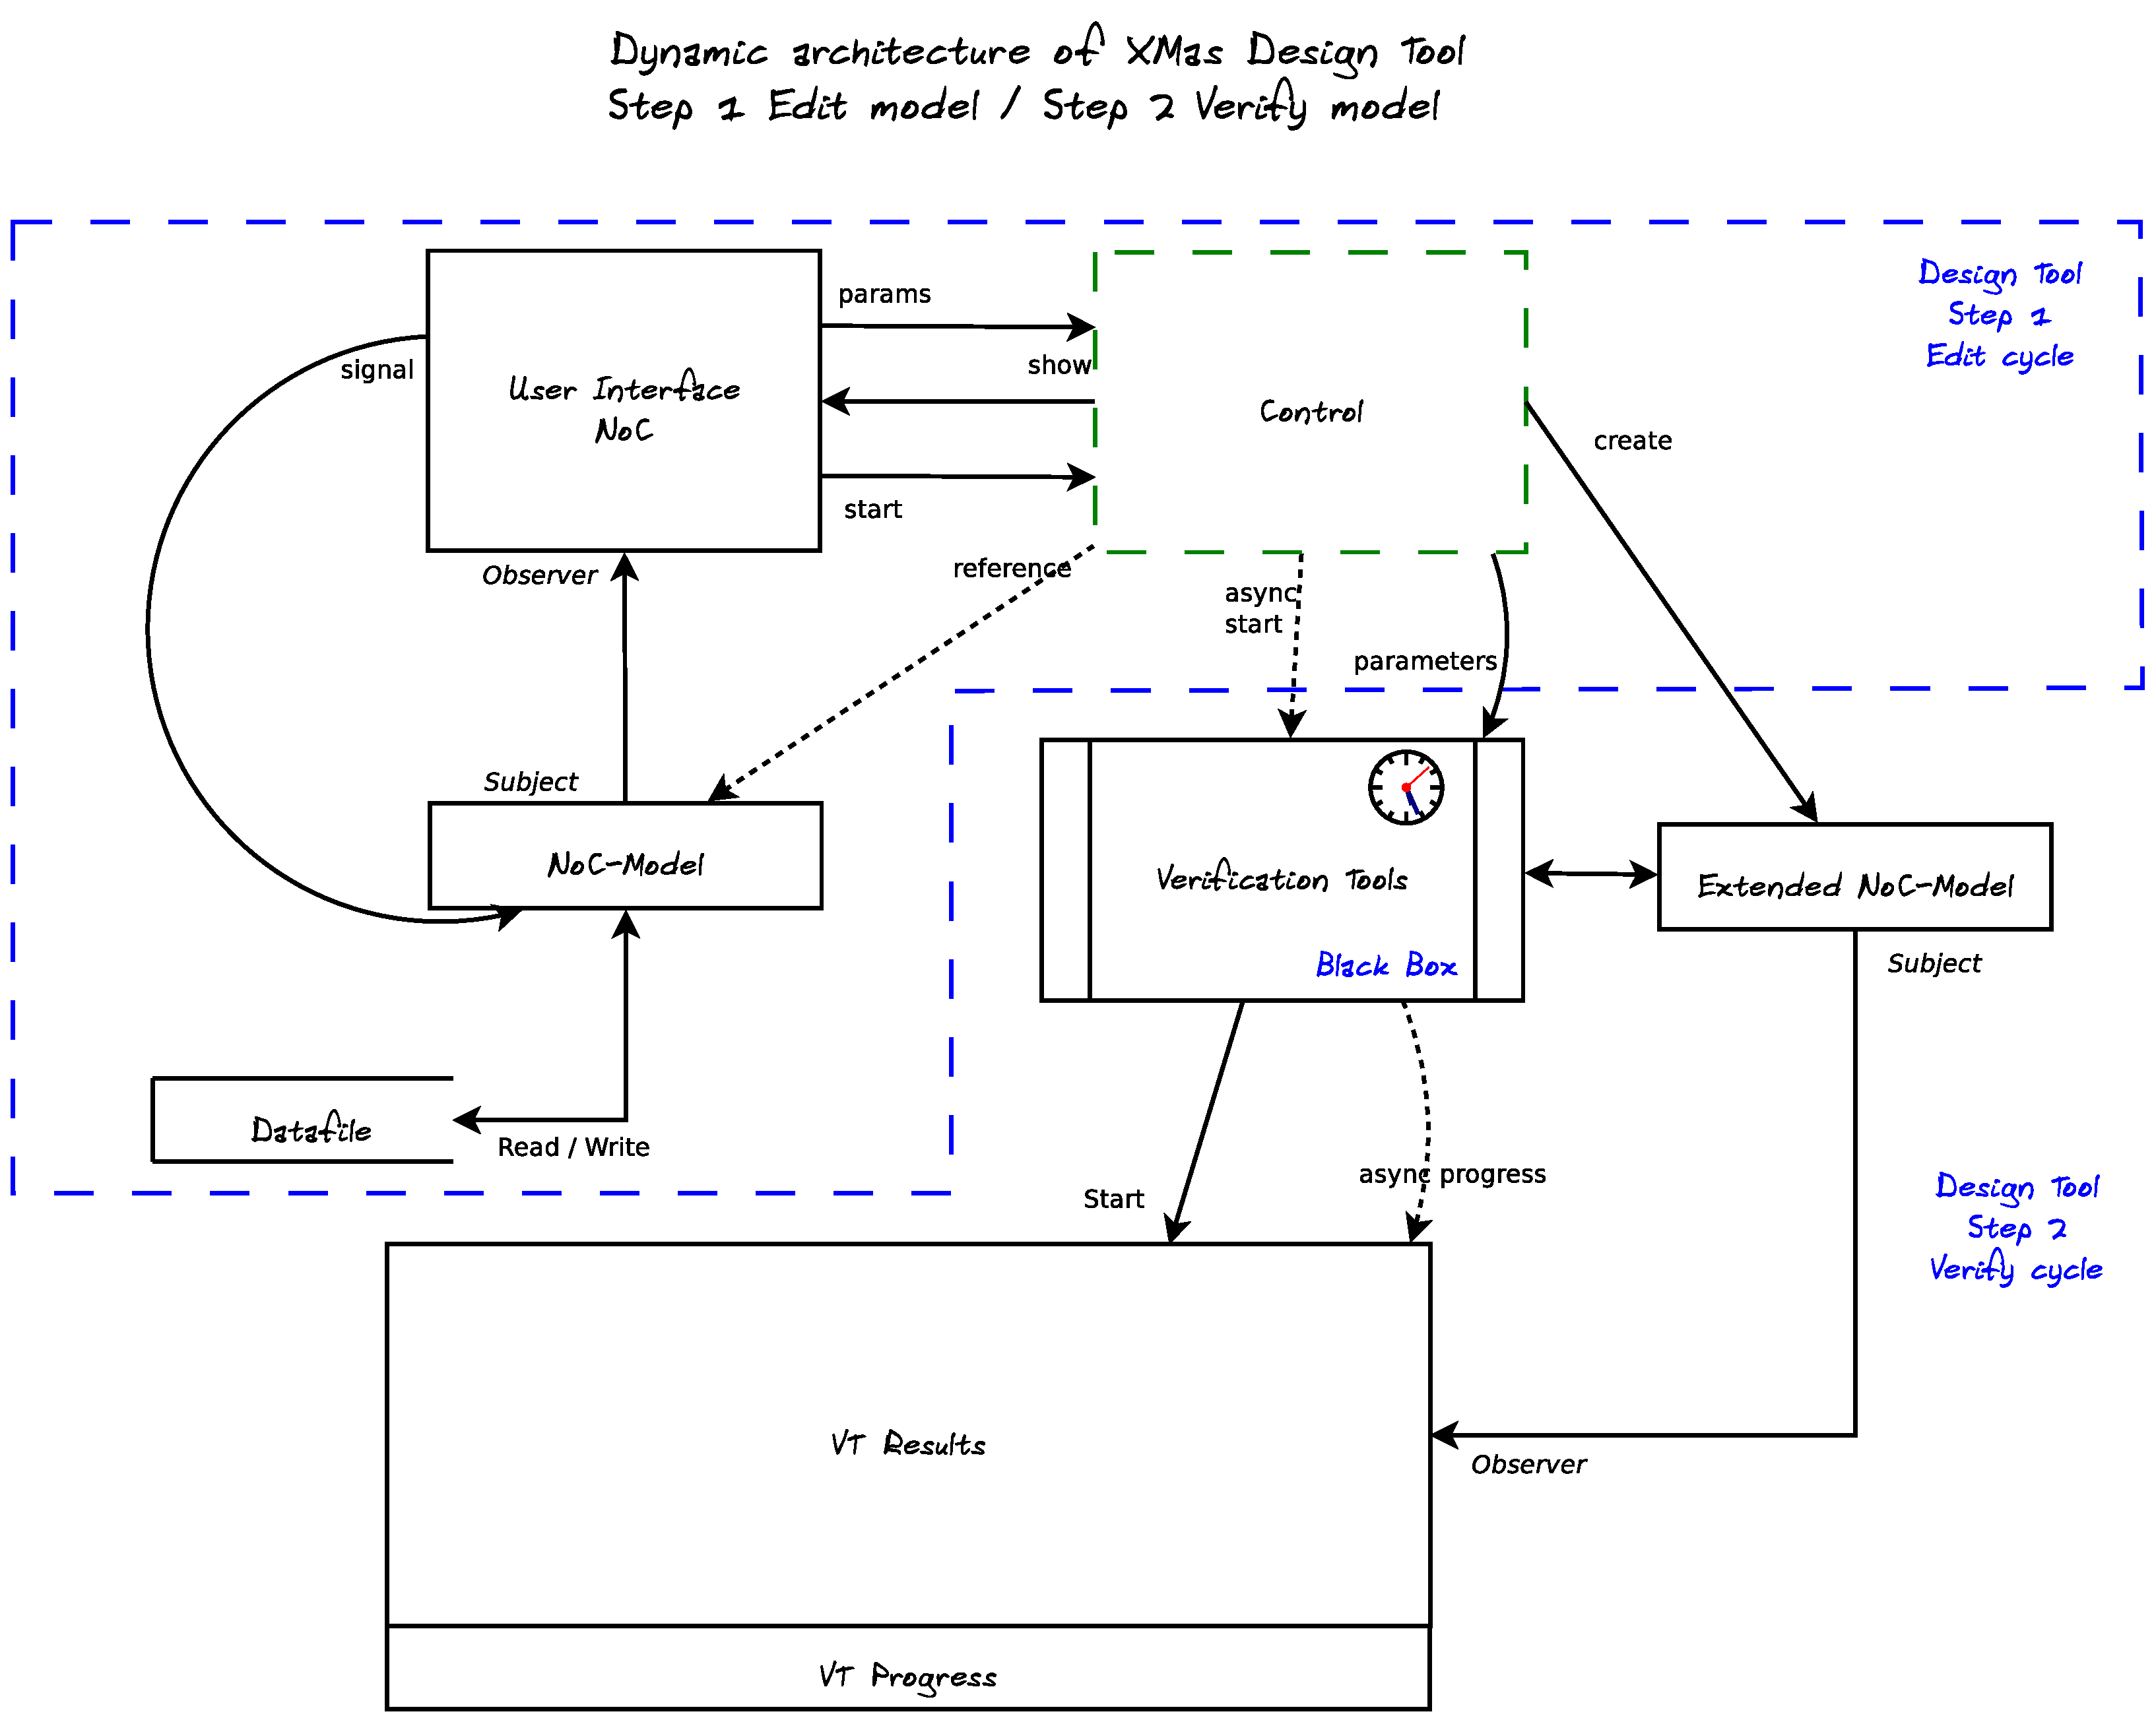
\includegraphics[width=.95\linewidth]{1c-architecture-dynamic}<7>
\end{frame}

\begin{frame}{Queries}
	\uncover<1>{\huge ?}
\end{frame}

\end{document}